% !TeX spellcheck = it_IT
\documentclass[10pt,a4paper]{article}

\usepackage[utf8]{inputenc}
\usepackage[T1]{fontenc}	
\usepackage[italian]{babel}
\usepackage{amsmath}
\usepackage{amsfonts}
\usepackage{amssymb}
\usepackage{graphicx}

\usepackage[left=2cm,right=2cm,top=2cm,bottom=2cm]{geometry}
\geometry{a4paper}

\usepackage{booktabs} % for much better looking tables
\usepackage{verbatim}
\usepackage{subfig} % make it possible to include more than one captioned figure/table in a single 

\usepackage{fancyhdr} % This should be set AFTER setting up the page geometry
\pagestyle{fancy} % options: empty , plain , fancy
\renewcommand{\headrulewidth}{0pt} % customise the layout...
\lhead{}\chead{}\rhead{}
\lfoot{}\cfoot{\thepage}\rfoot{}

%%% SECTION TITLE APPEARANCE
\usepackage{sectsty}
%\allsectionsfont{\sffamily\mdseries\upshape} % (See the fntguide.pdf for font help)
% (This matches ConTeXt defaults)

% pacchetti che mi fanno schifo ma uso lo stesso (Bob è scemo, ma anche Ale...)
\usepackage[cdot, thickqspace, squaren]{SIunits}
% il miglior pacchetto che potessi desiderare
\usepackage{float}
% macro che mi piacciono
\def\code#1{\texttt{#1}}


\title{Esercitazione 7: Amplificatore operazionale, usi non lineari}

\author{Gruppo BE \\ Alessandro Candido, Roberto Ribatti}
\date{\today}
\begin{document}
\maketitle

\section{Scopo e strumentazione}

\section{Discriminatore}

\section{Amplificatore di carica}

\section{Trigger di Schmitt}
Il trigger di Schmitt è costituito dal circuito in \figurename{~\ref{fig:schmitt_trigger}}.

\begin{figure}[H]
	\centering
	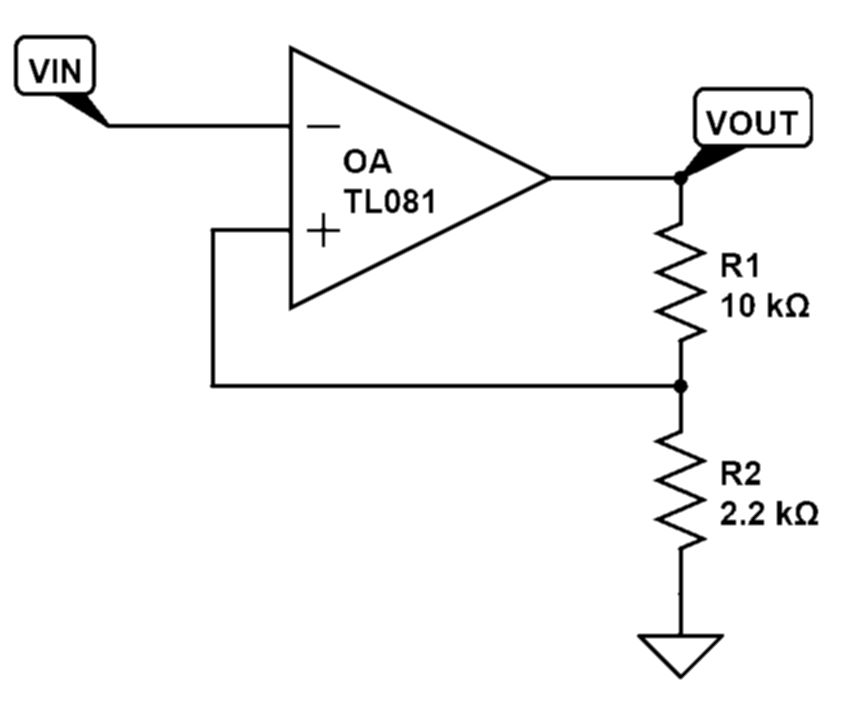
\includegraphics[width=0.40\textwidth]{../circuiti/schmitt_trigger.jpg}
	\caption{Schema del circuito del trigger di Schmitt}
	\label{fig:schmitt_trigger}
\end{figure}

I valori delle resistenze utilizzate sono riportati di seguito:

\begin{table}[H]
	\centering
	\begin{tabular}{cc}
        $ R_1 = \unit{9.88 \pm 0.08}{\kilo\ohm}$  & $R_2 = \unit{2.31 \pm 0.02}{\kilo\ohm}$
	\end{tabular}
\end{table}

Il grafico della risposta ad un segnale sinusoidale è riportato in \figurename{~\ref{fig:schmitt}}.

\begin{figure}[H]
    \centering
    \begin{minipage}{0.49\textwidth}
	    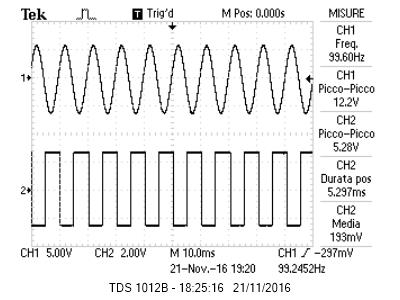
\includegraphics[width=\textwidth]{../oscilloscopio/schmitt.jpg}
	    \caption{Risposta ad un segnale sinusoidale}
	    \label{fig:schmitt}
    \end{minipage}
    \begin{minipage}{0.49\textwidth}
        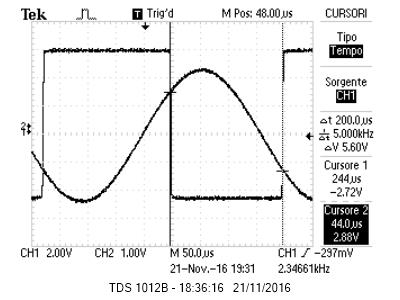
\includegraphics[width=\textwidth]{../oscilloscopio/schmitt_soglia.jpg}
        \caption{Misura delle tensioni di soglia}
        \label{fig:schmitt_soglia}
    \end{minipage}
\end{figure}

Il funzionamento del circuito osservato corrisponde a quanto atteso:
\begin{itemize}
\item il valore di $V_{out}$ è inizialmente fisso ad una delle due tensioni di alimentazione;
\item quando $V_{in}$ supera la corrispondente tensione di soglia $V_{out}$ scatta, e passa all'altra tensione di alimentazione;
\item quando $V_{in}$ supera la seconda soglia $V_{out}$ scatta nuovamente, e torna al valore iniziale.
\end{itemize}

I valori delle due soglie sono stati misurati, com'è mostrato in \figurename{~\ref{fig:schmitt_soglia}}, e vengono riportati di seguito:

\begin{table}[H]
	\centering
	\begin{tabular}{cc}
        $ V_{TH} = \unit{2.72 \pm 0.08}{\volt}$  & V_{TL} $\unit{-2.56 \pm 0.08}{\volt}$
	\end{tabular}
\end{table}

Mentre i valori fra cui oscilla $V_{out}$ sono:

\begin{table}[H]
	\centering
	\begin{tabular}{cc}
        $ V_{H} = \unit{14.0 \pm 0.4}{\volt}$  & $V_{L} = \unit{-13.4 \pm 0.4}{\volt}$
	\end{tabular}
\end{table}

\paragraph{Comportamento in ampiezza} Se si aumenta l'ampiezza del segnale in ingresso il funzionamento del circuito rimane qualitativamente lo stesso: per tensioni d'ingresso al di fuori dell'intervallo definito dalle due soglie il valore dell'uscita rimane costante (infatti non può superare il valore dell'alimentazione, né in positivo né in negativo). Per segnali di ampiezza sufficientemente bassa invece non si riesce a superare i valori di soglia, e l'uscita rimane fissa su una delle due tensioni di alimentazione.

\paragraph{Comportamento in frequenza} A bassa frequenza il circuito riproduce il comportamento ideale precedentemente descritto. Ad alta frequenza l'output è invece limitato dallo slew rate nelle transizioni tra i due stati, perciò quella che nel caso ideale dovrebbe essere un'onda quadra viene deformata, come risulta in \figurename{~\ref{fig:slew_rate}}, riprodotta di seguito.

\emph{Si nota che, come riportato da datasheet, lo slew rate in salita e in discesa non coincide, in particolare il primo è inferiore al secondo, con valori rispettivamente di $\unit{1.14 \pm 0.04}{\volt/\micro\second}$ e $\unit{1.30+/-0.04}{\volt/\micro\second}$, misurati ad una frequenza di $\unit{138 \pm 1}{\kilo\hertz}$}

\begin{figure}[H]
	\centering
	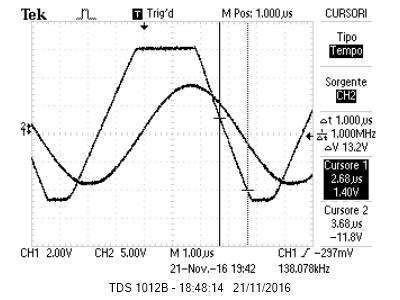
\includegraphics[width=0.40\textwidth]{../oscilloscopio/schmitt_slewrate.jpg}
	\caption{Effetto dello slew rate dell'OpAmp sull'output}
	\label{fig:slew_rate}
\end{figure}

%Si ha perciò che il comportamento del circuito è ideale per frequenze al di sotto di $\sim boh, non c'è scritto su misure$

% Problema: come diamine si giustifica la discesa più rapida dello slew_rate? Io ce la scriverei, ma due righe di ipotesi andrebbero scritte.

\section{Multivibratore astabile}
Il multivibratore astabile è costituito dal circuito in \figurename{~\ref{fig:multivibratore}}.

\begin{figure}[H]
	\centering
	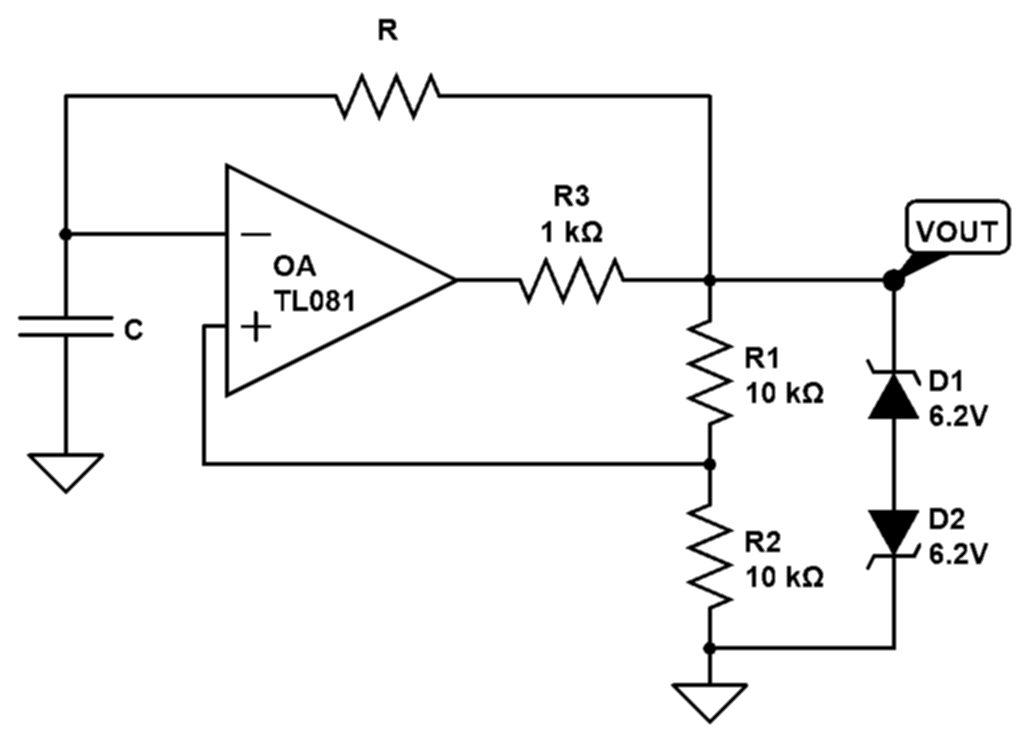
\includegraphics[width=0.40\textwidth]{../circuiti/multivibratore.jpg}
	\caption{Schema del circuito del multivibratore astabile}
	\label{fig:multivibratore}
\end{figure}

Come ricavato a lezione il periodo di oscillazione dell'output è pari a $T = 2 \tau \text{ln}(1 + 2 R_2/R_1)$, ed è indipendente dalla tensione di breakdown degli Zener $V_Z$.

Si sono scelti di conseguenza dei valori di $R$ e $C$ tali che il periodo fosse $\sim \unit{2}{\milli\second}$ come ricavato. I valori misurati, di questi e degli altri componenti, sono riportati di seguito.

\begin{table}[H]
	\centering
	\begin{tabular}{ccccc}
        $ R_1 = \unit{9.88 \pm 0.08}{\kilo\ohm}$ & $R_2 = \unit{9.88 \pm 0.08}{\kilo\ohm}$ & $R_3 = \unit{983 \pm 8}{\ohm}$ & $R = \unit{8.13 \pm 0.07}{\kilo\ohm}$ & $C = \unit{109 \pm 4}{\nano\farad}$
	\end{tabular}
\end{table}

\subsection{Analisi del funzionamento}
L'OpAmp amplifica qualunque minima differenza di tensione fra i due terminali di input, si avrà quindi che, non pilotando gli ingressi con alcuna tensione di input, qualche minima differenza di tensione, dovuta quindi al rumore, venga amplificata (è molto facile che già questo porti l'output a saturazione).

Si viene dunque a creare una differenza di potenziale ai capi della resistenza $R$ che induce una corrente e porta infine alla carica del condensatore $C$.

Il condensatore $C$, caricandosi, porterà a un certo punto la tensione al terminale '-' a oltrepassare, in positivo o in negativo a seconda dello stato di $V_{out}$, la tensione al terminale '+', necessariamente minore in modulo di $V_{out}$ in quanto determinata dal partitore $R_1 - R_2$.

Non appena avviene questo passaggio lo stato dell'ouput salta, e satura all'altro stato, determinando quindi un'inversione della corrente che scorre attraverso la resistenza $R$ e invertendo la carica del condensatore.

Raggiunta nuovamente la soglia determinata da $V_+$ l'output scatta di nuovo e cambia stato, e così via. Il tempo con cui avviene questo processo è quello riportato sopra nella formula per il periodo, ed è fissato dal tempo impiegato dal processo di carica del condensatore per raggiungere la soglia fissata da $V_+$, quindi come atteso dipenderà solamente dalla costante $\tau$ del circuito $R-C$ e dal rapporto di partizione del partitore $R_1-R_2$.

\subsection{Analisi dei segnali in ingresso e in uscita dall'OpAmp}
I segnali $V_+$, $V_-$ e $V_{out}$ sono rappresentati nelle figure~\ref{fig:multivibratore-} e \ref{fig:multivibratore+}, in particolare:
\begin{description}
\item[\figurename{~\ref{fig:multivibratore-}}] sono raffigurati i segnali $V_-$ e $V_{out}$, rispettivamente la \emph{pinna di squalo} e l'onda quadra;
\item[\figurename{~\ref{fig:multivibratore+}}] sono raffigurati i segnali $V_+$ e $V_{out}$, entrambi onde quadre, ma il primo è minore in modulo del secondo in entrambi gli stati a causa del partitore $R_1-R_2$.
\end{description}

\begin{figure}[H]
    \centering
    \begin{minipage}{0.49\textwidth}
        \centering
        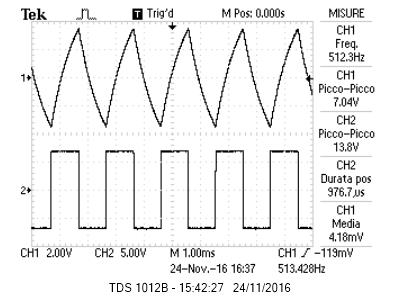
\includegraphics[width = \textwidth]{../oscilloscopio/multivibratore.jpg}
        \caption{Tensioni di output e al terminale '-' nel multivibratore}
        \label{fig:multivibratore-}
    \end{minipage}
    \begin{minipage}{0.49\textwidth}
        \centering
        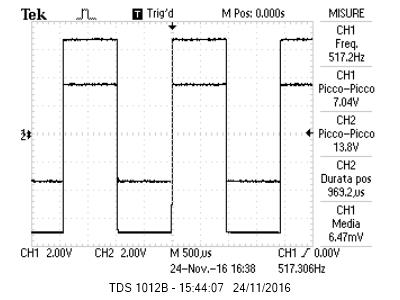
\includegraphics[width = \textwidth]{../oscilloscopio/multivibratore_V+.jpg}
        \caption{Tensioni di output e al terminale '+' nel multivibratore}
        \label{fig:multivibratore+}
    \end{minipage}
\end{figure}

I valori misurati per gli stati alto e basso dell'output e di $V_+$ sono:

\begin{table}[H]
	\centering
	\begin{tabular}{cc}
        $ V_{out H} = \unit{6.9 \pm 0.2}{\volt}$  & $V_{out L} = \unit{-6.9 \pm 0.2}{\volt}$\\
        $ V_{+ H} = \unit{3.52 \pm 0.11}{\volt}$  & $V_{+ L} = \unit{-3.52 \pm 0.11}{\volt}$
	\end{tabular}
\end{table}

\paragraph{$V_{out}} Che è consistente con quanto atteso. Infatti gli Zener hanno una tensione di breakdown pari a $\sim \unit{6.2}{\volt}$, aggiungendo $V_\gamma$ (cioè la tensione a cui il diodo passa in conduzione, o forward voltage), che da datasheet è al più $\unit{1.5}{\volt}$, si ha effettivamente la consistenza del valore misurato.

\paragraph{Zener e $R_3$} Quello che succede è che la tensione al terminale di output dell'OpAmp, dovuta all'alimentazione, è maggiore della massima caduta di tensione fissata dagli Zener. Per questo ai capi della resistenza $R_3$ si ha una data caduta di potenziale (che corrisponde a $V_{CC}-V_Z$), che porta ad una corrente che fluisce nella resistenza. In questo modo è possibile fissare il valore dei due stati di $V_{out}$ coi soli Zener, rendendo tali valori indipendenti dal valore dell'amplificazione dell'OpAmp e dall'alimentazione.

\paragraph{$V_+} Riguardo $V_+$ si ha che questo è determinato da $V_{out}$ e dal rapporto di partizione $R_1 - R_2$, che in questo caso, poiché $R_1 \sim R_2$ è circa la metà. Per l'esattezza il rapporto di partizione atteso è pari a $\unit{0.5000 \pm 0.0028}$ mentre il rapporto fra le due tensioni misurate è pari a $\unit{0.510 \pm 0.022}$, e quindi i due valori sono compatibili.
Per l'esattezza l'espressione che si ottiene dalla teoria per i due punti di inversione è $V_Z R_2/(R_1 + R_2)$.

\paragraph{$V_-} Si discute infine del segnale $V_-$.
Questa segnale, come già detto e come si può osservare dalla \figurename{~\ref{fig:multivibratore-}, è una tipica onda a \emph{pinna di squalo}, cioè la successione di esponenziali crescenti e decrescenti, dovuti alle cariche e scariche del condensatore $C$. I valori misurati per le tensioni nei punti d'inversione sono $\pm \unit{3.52 \pm 0.11}{\volt}$.
La tensione nei punti di inversione è dunque esattamente la stessa che si ha per $V_+$, come atteso dato l'altissimo valore di amplificazione dell'OpAmp.

\subsection{Dipendenza del periodo di $V_{out}$ dalla tensione di alimentazione}

\subsection{Limiti in frequenza dell'onda quadra generata}


\pagebreak
\section{Appendice: Dati acquisiti}
Si riportano qui le tabelle dei dati usati per i fit e i grafici.

%\centering
%\begin{figure}[h!]
%	\begin{minipage}[t]{0.33\textwidth}
%		\resizebox{1\textwidth}{!}{
%		\input{../tabelle/tab_inv_amp_gain.txt}}
%		\captionof{table}{Guadagnio amplificatore invertente}
%		\label{tab:inv_amp_gain}
%	\end{minipage}
%	\begin{minipage}[t]{0.33\textwidth}
%		\resizebox{1\textwidth}{!}{
%		\input{../tabelle/tab_inv_amp_f_domain.txt}}
%		\captionof{table}{Risposta in frequenza amplificatore invertente}
%		\label{tab:inv_amp_f_domain}
%	\end{minipage}
%	\begin{minipage}[t]{0.33\textwidth}
%		\resizebox{1\textwidth}{!}{
%			\input{../tabelle/tab_gain_bandwidth.txt}}
%		\captionof{table}{Banda/Guadagno}
%		\label{tab:gain_bandwidth}
%	\end{minipage}
%\end{figure}

%\begin{figure}[h!]
%	\centering
%	\resizebox{0.7\textwidth}{!}{
%	\input{../tabelle/tab_low_pass.txt}}
%	\captionof{table}{Dati relativi al circuito integratore}
%	\label{tab:lowpass}
%\end{figure}

%\begin{figure}[H]
%	\centering
%	\resizebox{0.7\textwidth}{!}{
%	\input{../tabelle/tab_high_pass.txt}}
%	\captionof{table}{Dati relativi al circuito derivatore}
%	\label{tab:highpass}
%\end{figure}



\end{document}
